\chapter{Lecture 12}

%--- 信息 ----
\begin{center}
    讲师:王立威 \qquad
    课程时间:25.May.13rd \qquad 
    笔记:25.June.9th
\end{center}

\bigskip

首先引入概念
\begin{definition}[码率]
    一个信道通信的\textbf{码率}(rate)是指平均每次传输有效信息量.
\end{definition}
\begin{example}
    如果我传输一个比特时,将其重复$n$次再传输,那么码率为$1/n$.
\end{example}

然后叙述一直以来想要证明的重要定理:
\begin{theorem}[Shannon 信道编码定理]
    对于一个含噪信道,记其信道容量为$C$,希望码率为$R$. 那么 
    \begin{itemize}
        \item 若$R < C$,那么对于任意$\varepsilon > 0$存在码率至少为$R$的纠错码,使得错误概率小于$\varepsilon$.
        \item 若$R > C$,那么存在$\varepsilon_0 > 0$,对于任意码率至少是$R$的纠错码其错误概率都至少是$\varepsilon_0$.
    \end{itemize}
\end{theorem}
\begin{proof}
    我们这里主要阐述Shannon精妙的思想,后续严格化工作请自行补充.  
    \begin{enumerate}
        \item[(1)] $R<C$时. 不失一般性(这里需要思考),假设信息集为$\{m_1,m_2,\dots, m_{nR}\}$并且它们均匀分布. 下面来设计码字集合$(c_1,c_2,\dots, c_{nR})$ 
        
        使用随机编码(考虑所有可能的码字集合),设每个码字长度都为$n$,记 
        \[
        c_i = (c_{i1}, c_{i2},\dots, c_{in}), \quad i = 1,2,\dots 2^{nR}
        \]

        由于信息的熵为$nR$,码字长度为$n$,所以码率为$R$。

        根据信道容量的定义,取使得达到信道容量的先验分布:
        \[
        P(X) = \mathop{\arg\max}_{P_X} I(X;Y)
        \]

        我们现在令$c_{ij}$独立同分布地服从分布$P(X)$(对于所有$i,j$)这一步是整个证明中很关键的一步!我们考察其平均错误率,如果平均错误率$< \varepsilon$,那么就一定有一组码字的错误率$< \varepsilon$.  不过我们仍需给出解码的方法。

        解码时,当我们接收到$(y_1, \dots, y_n)$时。我们将其对应到$c_i = (x_1, \dots, x_n)$使得$(x_1,\dots, x_n; y_1,\dots, y_n)$是关于联合分布$P(X)P(Y|X)$的典型序列;如果没有这样的或者有多于一个的$(x_1,\dots, x_n)$,那么返回错误;如果唯一存在$c_i$,则返回$c_i$。

        下面计算错误概率,不妨假设我们原定传输的信息是$m_1$
        \[
        \Pr\Big[\text{找到多个解}\Big] \le \sum_{i=2}^{2^{nR}} \Pr\Big[\bm{y}\text{和}c_i\text{匹配为典范序列}\Big] \approx 2^{nR} \cdot 2^{-n I(X;Y)}
        \]

        而根据我们的$P(X)$的选择,会有$I(X;Y) = C$,上式右侧变为$2^{n(R-C)}$,所以当$R<C$时取$n$充分大即可. 而 
        \[
        \Pr\Big[\text{找不到解}\Big] \le \varepsilon
        \]

        所以加在一起的错误概率就是趋于零的,因此可以任意小. 

        \item[(2)] 当$R > C$时,往证明存在$\varepsilon_0$使得任意纠错码的错误率都$\ge \varepsilon_0$. 我们需要使用Fano不等式(写在后面)
        
        设我们发出的消息是$M$,收到比特流$Y_1,\dots, Y_n$,则 
        \[
        H(M|Y_1,\dots Y_n) = H(X) - I(M;Y_1,\dots, Y_n) \ge nR - nC = n(R-C)
        \] 

        那么错误概率
        \[
        P_{\text{error}} \ge \dfrac{H(M|Y_{1\sim n}) - 1}{\log \abs{\{0,1\}^{nR}}} \ge \dfrac{n(R-C) - 1}{nR} = \dfrac{R-C}{R} - O(n^{-1})
        \]

        可以看出错误率存在正下界. 
    \end{enumerate}

    综合两部分便完成了定理的证明.
\end{proof}

\begin{theorem}[Fano不等式]
    令$X,Y$是随机变量,$X \in \cal{H}$,其取值范围有限$\abs{\cal{H}} < \infty$。 现在我们使用$Y$来估计$X$,记估计值$\hat{X} = g(Y)$,那么错误概率满足 
    \[
    P_{\text{error}} = \Pr[\hat{X} \neq X] \ge \dfrac{H(X|Y) - 1}{\log \abs{\cal{H}}}
    \]
\end{theorem}
% \begin{figure}[H]
%     \centering
%     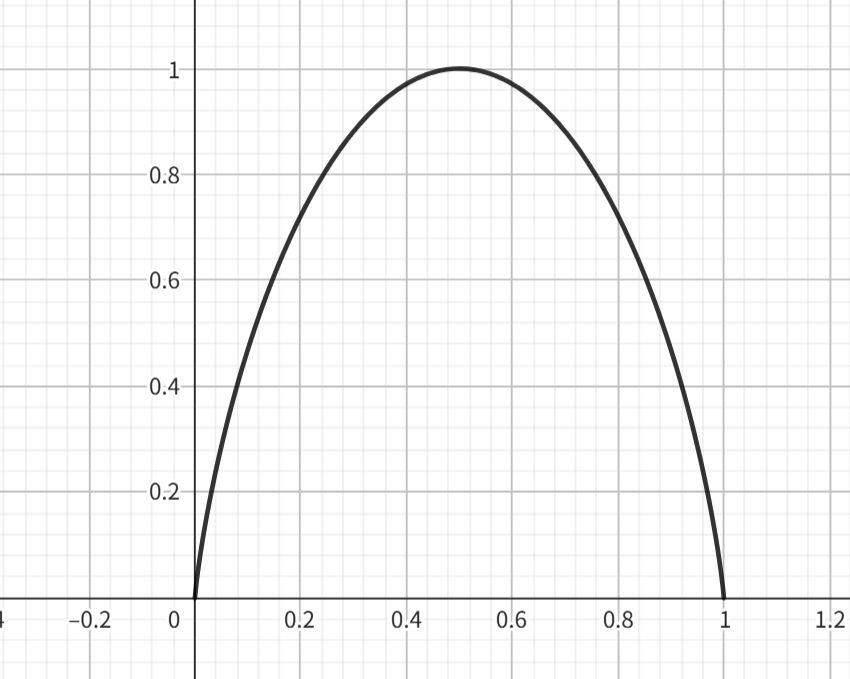
\includegraphics[width=.6\textwidth]{images/c2_1.png}
%     \caption{$H=x\log 1/x + (1-x)\log 1/(1-x)$的图像}
% \end{figure}